\documentclass[12pt]{article}
\usepackage[margin=1in]{geometry}

% Start of preamble
%==========================================================================================%
% Required to support mathematical unicode
\usepackage[warnunknown, fasterrors, mathletters]{ucs}
\usepackage[utf8x]{inputenc}

% Always typeset math in display style
%\everymath{\displaystyle}

% GROUPOIDS FONT!
\usepackage{eulervm}
\usepackage{charter}

% Standard mathematical typesetting packages
\usepackage{amsthm, amsmath, amssymb}
\usepackage{mathtools}  % Extension to amsmath

% Symbol and utility packages
\usepackage{cancel, textcomp}
\usepackage[mathscr]{euscript}
\usepackage[nointegrals]{wasysym}

% Extras
\usepackage{physics}  % Lots of useful shortcuts and macros
\usepackage{tikz-cd}  % For drawing commutative diagrams easily
\usepackage{color}  % Add some color to life
\usepackage{microtype}  % Minature font tweaks
%\usepackage{pgfplots} % plots

\usepackage{enumitem}
\usepackage{titling}

\usepackage{graphicx}

% Common shortcuts
\def\mbb#1{\mathbb{#1}}
\def\mfk#1{\mathfrak{#1}}

\def\bN{\mbb{N}}
\def\bC{\mbb{C}}
\def\bR{\mbb{R}}
\def\bQ{\mbb{Q}}
\def\bZ{\mbb{Z}}

% Sometimes helpful macros
\newcommand{\floor}[1]{\left\lfloor#1\right\rfloor}
\newcommand{\ceil}[1]{\left\lceil#1\right\rceil}
\DeclarePairedDelimiterX\set[1]\lbrace\rbrace{\def\given{\;\delimsize\vert\;}#1}

% Some standard theorem definitions
\newtheorem{theorem}{Theorem}[section]
\newtheorem{corollary}{Corollary}[theorem]
\newtheorem{lemma}[theorem]{Lemma}

\theoremstyle{definition}
\newtheorem{definition}{Definition}[section]

\theoremstyle{remark}
\newtheorem*{remark}{Remark}

% End of preamble
%==========================================================================================%

% Start of commands specific to this file
%==========================================================================================%

\newcommand{\R}{\mathbb{R}}
\renewcommand{\ip}[2]{\langle #1, #2 \rangle}
\newcommand{\mg}[1]{\| #1 \|}
\newcommand{\linf}[1]{\max_{1\leq i \leq #1}}
\newcommand{\ve}{\varepsilon}
\renewcommand{\qed}{\hfill\qedsymbol}
\newcommand{\seq}[2]{\qty(#1_#2)_{#2=1}^{\infty}}
\newcommand{\justif}[1]{&\quad &\text{(#1)}}
\newcommand{\ra}{\rightarrow}


%==========================================================================================%
% End of commands specific to this file

\title{CSE 311 HW 2}
\date{\today}
\author{Rohan Mukherjee}

\begin{document}
	\maketitle
	\begin{enumerate}[leftmargin=\labelsep]
		\item 
		\begin{enumerate}
			\item The intuition that I am going with is that the first two pieces are independent of the value of $p$, as either $p$ or $\lnot p$ is true. So the first two pieces are really only true if $q$ is true, as you would have $(F \land q) \lor (T \land q)$ given any truth value of $p$. 
			\item 
			\begin{alignat*}{2}
				(p \land q) \lor (\lnot p \land q) \lor (\lnot p \land \lnot q) &\equiv (q \land p) \lor (q \land \lnot p) \lor (\lnot q \land \lnot p) \justif{Commutativity 3 times} \\
				&\equiv [q \land (p \lor \lnot p)] \land (\lnot q \land \lnot p) \justif{Distributivity} \\
				&\equiv [q \land T] \lor (\lnot p \land \lnot q) \justif{Absorption} \\
				&\equiv q \lor (\lnot p \land \lnot q) \justif{Identity} \\
				&\equiv (q \lor \lnot p) \land (q \lor \lnot q) \justif{Distributivity} \\
				&\equiv (q \lor \lnot p) \land T \justif{Negation} \\
				&\equiv q \lor \lnot p \justif{Identity} \\
				&\equiv \lnot p \lor q \justif{Commutativity} \\
				&\equiv p \ra q \justif{Law of implication}
			\end{alignat*}
			\item Step 1-3 is doing what we discussed for the intuition, simplifying the first two parts to just $q$. Steps 4-5 are trying to get rid of the $\lnot q$, because it actually doesn't add anything to the final answer. Then the last step is just using the law of implication to finish off the proof.
		\end{enumerate}
	
	\newpage
	\item 
	\begin{enumerate}
		\item $z \lor \lnot y$.
		\item $\lnot z \lor x$
		\item 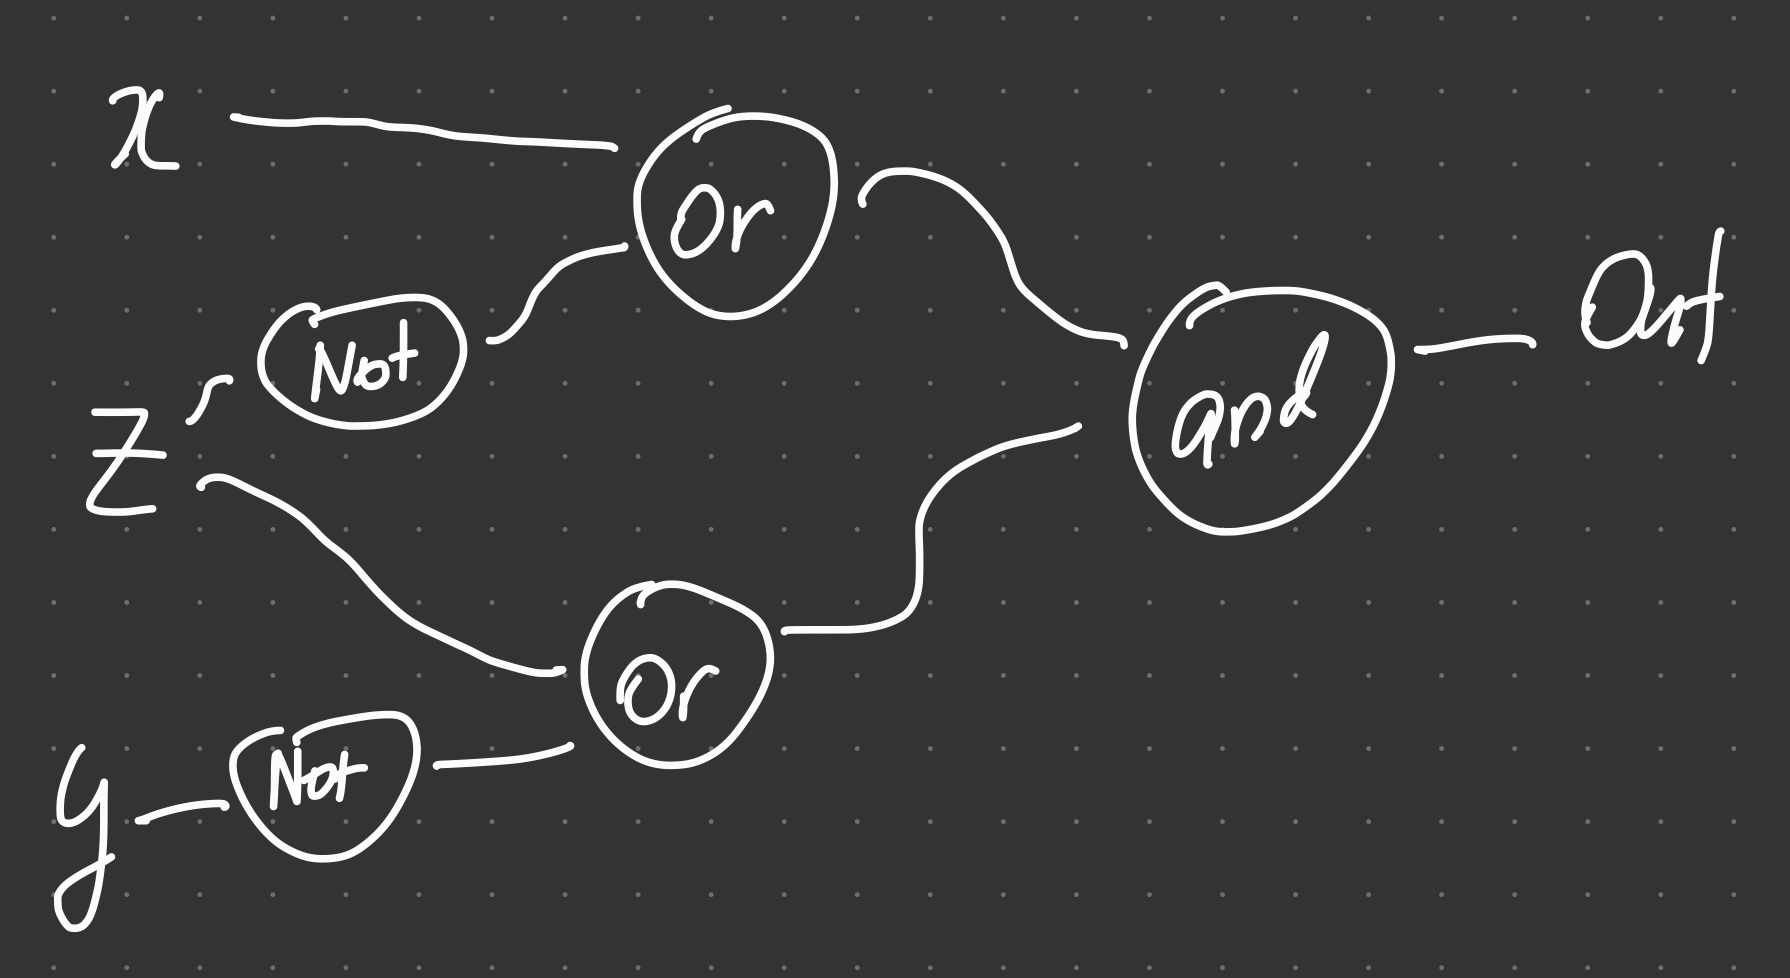
\includegraphics[scale=0.15]{circuit.png}
	\end{enumerate}

	\newpage
	\item 
	\begin{enumerate}
		\item 
		\begin{enumerate}
			\item Let $p = $ you can easily become a multi-millionaire, $q = $ you can take an infinitely long vacation at Cancun resort $r = $ you solve one of the Millennium Problems. We have $r \ra (p \land q)$.
			\item 
			$(\lnot p \lor \lnot q) \ra \lnot r$.
			\item If you aren't a millionaire, or you can't take an infinitely long vacation at Cancun resort, then you haven't solved a Millennium problem.
			\item Yes.
		\end{enumerate}
		\item 
		\begin{enumerate}
			\item Let $q = $ we design a better model, and $p = $ we will reach artificial general intelligence. We have $\lnot q \ra \lnot p$.
			\item 
			$p \ra q$. 
			\item We reached artificial general intelligence only if we designed a better model.
			\item Yes.
		\end{enumerate}
	\end{enumerate}

	\newpage
	\item 
	\begin{enumerate}
		\item $a \land (b \lor (\lnot b \lor a)) \lor \lnot(a \land (a \lor b))$
		\item \begin{alignat*}{2}
			\lnot (a \land (a \lor b)) &\equiv \lnot a \lor \lnot(a \lor b) \justif{Demorgans} \\
			&\equiv \lnot a \lor (\lnot a \land \lnot b) \justif{Demorgans} \\
			&\equiv (\lnot a \lor \lnot a) \land (\lnot a \lor \lnot b) \justif{Distributivity} \\
			&\equiv \lnot a \land (\lnot a \lor \lnot b) \justif{Idempotency} \\
			&\equiv (\lnot a \land \lnot a) \lor (\lnot a \lor \lnot b) \justif{Distributivity} \\
			&\equiv \lnot a \lor (\lnot a \lor \lnot b) \justif{Idempotency}
		\end{alignat*}
		\begin{alignat*}{2}
			a \land (b \lor (\lnot b \lor a)) &\equiv a \land ((b \lor \lnot b) \lor a) \justif{Associativity} \\
			&\equiv a \land (T \lor a) \justif{Negation} \\
			&\equiv a \land T \justif{Domination} \\
			&\equiv a \justif{Identity}
		\end{alignat*}
		\begin{alignat*}{2}
			a \land (b \lor (\lnot b \lor a)) \lor \lnot(a \land (a \lor b)) &\equiv a \lor (\lnot a \lor (\lnot a \lor \lnot b)) \justif{Look up!} \\
			&\equiv (a \lor \lnot a) \lor (\lnot a \lor \lnot b) \justif{Associativity} \\
			&\equiv T \lor (\lnot a \lor \lnot b) \justif{Negation} \\
			&\equiv T \justif{Domination}
		\end{alignat*}
	\item We know that the boolean algebra expression will evaluate to true because in any case, if $A = 0$ then the second quantity will be $1$, and adding $1$ forces the entire statement to be 1 (in the proof, this is where we have $\lnot a \lor$). If $A = 1$, then the first quantity $= 1$, as in the proof we showed the first statement was $= A$. As $A$ will be either 1 or 0, this shows that the above statement is a tautology (also, there is a $+$ between the two quantities, so if either are 1 then the whole thing is too)
	\end{enumerate}

	\newpage
	\item
	\begin{enumerate}
		\item Let $P(x) = x$ is even and $Q(x) = x$ is odd, and the domain of discourse be $\bZ$. Then $\forall x(P(x) \lor Q(x))$ is equivalent to the statement that "every integer is either odd or even", which is clearly true. However, $\forall x (P(x)) \lor \forall x (Q(x))$ is equivalent to the statement "every integer is even or every integer is odd", which is not true. 
		\item Let $P(x) = x$ is an integer, $Q(x) = x$ is not an integer, and the domain of discourse be $\bZ$. Then $\forall x(P(x) \lor Q(x))$ translates to every integer is either an integer or not an integer, which is clearly true. $\forall x (P(x)) \lor \forall x(Q(x))$ translates to every integer is an integer or every integer is not an integer, which is clearly also true. Because these have the same truth value, they are logically equivalent.
	\end{enumerate}

	\newpage
	\item 
	\begin{enumerate}
		\item As $P(x)$ is not always true, we can find an $x^*$ so that $P(x^*) = F$. Then clearly, we have found an $x^*$ so that $P(x^*) \ra Q(x^*)$ is true, as $F \ra Q(x) \equiv T$. So the original statement is true.
		\item As $P(x)$ is always true, we can substitute in $T$ for it: $\exists x (T \ra Q(x)) \equiv \exists x (Q(x))$ (the latter statement is my answer). This works as $T \ra Q(x) \equiv \lnot T \lor Q(x) \equiv F \lor Q(x) \equiv Q(x)$.
	\end{enumerate}

	\newpage
	\item This took me around 3 hours. I spent the most time on problem 5, as it was really confusing. At least I learned that two statements including quantifiers are logically equivalent iff they hold the same truth value in every domain of discourse. I have no other feedback.
	\end{enumerate}
\end{document}